\documentclass[a4paper,11pt]{article}
\usepackage[utf8]{inputenc}
\usepackage[spanish]{babel}
\usepackage{setspace}
\usepackage{apalike}
\usepackage{cite}
\usepackage[pdftex]{graphicx}
\bibliographystyle{apalike}
\begin{document}
\title{\Huge Estimación de la edad a partir de restos esqueléticos}
\author{Guillermo Ramírez García}
\date{\today}
\maketitle
\newpage
\spacing{1.5}
\part{Introducción}
Esto se debe a que, en las primeras edades de la vida, los cambios óseos están mejor sistematizados, por tratarse de un periodo de desarrollo y, por tanto, de cambios continuos \cite{scheuer2004juvenile}.

Por otra parte, aunque pueden existir variaciones en el ritmo de crecimiento entre unas poblaciones y otras, el grado de variabilidad no es muy amplio, por lo que las estimaciones suelen ser bastante acertadas.

Para reconstruir los patrones de las sociedades del pasado se siguen los mismos fundamentos que utiliza la Demografía; la única diferencia es que, en estos casos, se trabaja con poblaciones muertas, por lo que datos relativos a curvas de mortalidad o estimaciones sobre esperanza media de vida al momento del nacimiento se realizan en intervalos de cinco años, mientras que en la actualidad se hacen de año en año.

En Antropología Forense, la estimación de la edad se aplica, por lo general, en restos óseos o en cadáveres en avanzado estado de descomposición, para estimar la edad que tenía una persona al morir, con el objeto de contribuir a su identificación; no obstante, también se utiliza de forma habitual en los subadultos para la estimación de la edad de personas vivas, con el objeto de ubicar a un individuo en un marco legal; por ejemplo, en casos de inmigración, infanticidio, pedofilia, etc.
            
La metodología empleada para la determinación de la edad en Antropología Física, está basada en la evaluación del estado de desarrollo de un esqueleto, o edad fisiológica, y la correspondencia de ésta con la edad cronológica; a continuación se definen cada una de ellas.
La metodología empleada para la determinación de la edad en Antropología Física, está basada en la evaluación del estado de desarrollo de un esqueleto, o edad fisiológica, y la correspondencia de ésta con la edad cronológica:
\begin{itemize}
\item {\bf Edad fisiológica:} es la edad que refleja el estado fisiológico de un individuo. Se define según criterios de maduración y desarrollo en individuos infantiles y a partir de la evaluación de signos degenerativos en indivudos adultos. En el contexto de la Antropología Física, la edad fisiológica distingue entre la “edad dental” y la “edad esquelética”.
\item {\bf Edad cronológica:} está únicamente determinada por la fecha de nacimiento y de defunción. En los casos de identificación forense, se dispondrá de este dato como parte de la información {\em antemortem} y será proporcionado por los familiares, o a partir de documentos oficiales; así mismo, en caso de conocerse, será el criterio empleado para ubicar al individuo de acuerdo a las diferentes edades de transición establecidas por la ley, condicionando así la aplicación de leyes y derechos.
\end{itemize}
Para poder estimar la edad de un individuo en el contexto de la Antropología Forense de una forma eficiente y responsable, ya sea a partir de unos restos óseos o en sujetos vivos, el antropólogo deberá poseer unos conocimientos específicos y amplios en las siguientes materias:
\begin{itemize}
\item Anatomía esquelética y dental, tanto infantil como adulta.
\item Rangos normales de variación humana, esqueléticos y dentales.
\item Rasgos patológicos que puedan afectar a la aplicación del método.
\item Experiencia en la manipulación de material osteológico.
\item Conocimiento actualizado y experiencia en la aplicación de las diferentes metodologías existentes.
\item Capacidad para evaluar los diferentes indicadores de edad y sus criterios estadísticos.
\end{itemize}

\part{Metodología}
\section{Conceptos importantes}
El grado de ajuste entre la edad cronológica y fisiológica que ofrece un determinado método, debe ser evaluado y cuantificado; además, debe incluir información detallada referente al margen de error Intra-observador e Inter-observador asumido. Por un lado, esto permitirá al antropólogo la elección correcta del método que más se ajuste a las circunstancias específicas de su estudio y, por otro lado, se trata de un valor que deberá ser incorporado en el informe antropológico como requisito indispensable cuando se trabaje en contextos forenses, ofreciendo el valor de la edad estimada como un intervalo de confianza y con una determinada probabilidad de acierto.
\subsection{Precisión y exactitud}
En ciencia, se emplean ambos conceptos para describir la relación entre un valor numérico estimado con su valor real correspondiente. En la temática que aquí se trata, equivale a la relación entre la edad estimada a partir de un determinado método y la edad real del individuo. Se trata de dos conceptos independientes que, en el lenguaje cotidiano, son empleados como sinónimos pero, cuando se emplean en un lenguaje técnico, ofrecen información muy diferente:
\begin{itemize}
\item {\bf La precisión} informa sobre la dispersión de los resultados obtenidos cuando se aplica un determinado método repetidas veces, sobre una misma población de individuos con características similares. En el caso de la estimación de la edad, informa sobre el margen de error asumido por dicho método, expresado en forma de intervalo de edad estimada, dentro del cual existe una determinada probabilidad de que esté representado el valor de la edad real. Cuanto más preciso sea un método, menor será el intervalo de edad estimada que ofrezca.
\item {\bf La exactitud} informa sobre la desviación del valor estimado por un determinado método con respecto al valor real. En el caso de la estimación de la edad, equivale a la probabilidad de que la edad real del individuo se encuentre dentro del intervalo de edad estimada ofrecida por el método.
\end{itemize}
Ambos conceptos dependen de factores diferentes, por lo que pueden ser utilizados de forma conjunta para informar sobre la aplicabilidad de un determinado método.
\begin{enumerate}
\item {\bf Método poco preciso y muy exacto:} en este caso, el intervalo de edad estimada sería muy amplio, no obstante, éste contendría la edad real con una probabilidad muy elevada. Esta situación podría producirse, por ejemplo, al emplear un método que fue diseñado, combinando la información de diversas poblaciones muy diferentes entre sí.
\begin{figure}[h!]
\centering
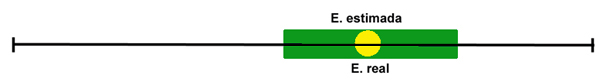
\includegraphics[scale=2]{1.jpg}
\end{figure}
\item {\bf Método poco preciso y poco exacto:} el intervalo de edad ofrecido sería muy pequeño; no obstante, la probabilidad de que la edad real se encontre dentro de dicho intervalo sería muy reducida. Este caso se produce, por ejemplo, cuando se aplican métodos que utilizan variables métricas muy precisas, pero que han empleado un volumen de muestra muy reducido para su diseño, por lo que no contemplan la variabilidad del rasgo analizado.
\begin{figure}[h!]
\centering
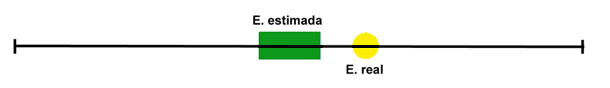
\includegraphics[scale=2]{2.jpg}
\end{figure}
\item {\bf Método muy preciso y muy exacto:} el intervalo de edad estimada es muy reducido y posee una gran probabilidad de incluir el valor de la edad real. Se trata de las características ideales que debe poseer un método para su aplicación en contextos forenses. Este caso se pude producir, por ejemplo, al emplear métodos que utilizaron grandes muestras de estudio para ser diseñados, que analicen variables métricas muy precisas y aplicados en la misma población que les dio origen.
\begin{figure}[h!]
\centering
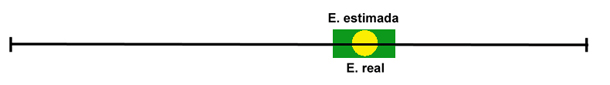
\includegraphics[scale=2]{3.jpg}
\end{figure}
\item {\bf Método poco preciso y poco exacto:} al contrario que el caso anterior, el intervalo de edad estimada es muy amplio y, además, existe una probabilidad reducida de que albergue la edad real. En este caso, podría mencionarse como ejemplo, un método que analice una variable débilmente relacionada con la edad del individuo.
\begin{figure}[h!]
\centering
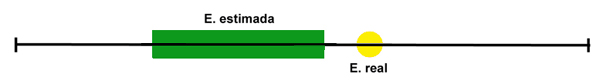
\includegraphics[scale=2]{4.jpg}
\end{figure}
\end{enumerate}

\subsection{Sensibilidad y especificidad}
En ocasiones, se emplean metodologías que no ofrecen como resultado un valor numérico, sino que informan sobre la posibilidad de que se cumpla, o no, una determinada condición, por lo que los únicos resultados posibles serán “sí” o “no”. En el contexto de la estimación de la edad, se trata de metodologías que evalúan determinados acontecimientos discretos en el proceso de maduración del esqueleto, para inferir si el individuo ha superado, o no, una edad concreta. Como ejemplos más destacados se pueden mencionar la unión de las epífisis de los huesos largos, la erupción dental, obliteración de las suturas craneales, etc.

En estos casos, los conceptos de sensibilidad y especificidad, se emplean para evaluar la validez del método, es decir, su capacidad para ubicar a cada individuo en su grupo de edad correspondiente, en función del resultado positivo, o negativo que se desprenda tras aplicar el método. Para explicar ambos conceptos se puede plantear como ejemplo la evaluación de un método antropológico cuyo objetivo es estimar si un individuo es mayor de edad, es decir, posee más de 18 años:
\begin{itemize}
\item {\bf Sensibilidad:} se define como la capacidad del método para detectar positivos, es decir, para identificar aquellos individuos que son mayores de 18 años.
\item {\bf Especificidad:} se define como la capacidad del método para detectar negativos, es decir, para identificar aquellos individuos que son menores de 18 años.
\end{itemize}
Aunque parezcan similares, ambos conceptos son complementarios y cada uno informa sobre una característica diferente del método. A continuación se muestran las 4 combinaciones posibles que se pueden realizar, empleando valores extremos, aplicadas al ejemplo anterior de un método cuyo fin es estimar la mayoría de edad:
\begin{enumerate}
\item {\bf Método muy sensible y muy específico:} posee una alta capacidad para detectar tanto positivos como negativos, por lo que es capaz de separar de manera muy eficiente a los individuos mayores de edad de los menores.
\begin{figure}[h!]
\centering
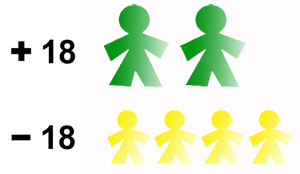
\includegraphics[scale=2]{5.jpg}
\end{figure}
\item {\bf Método muy sensible y poco específico:} alta capacidad para detectar positivos pero poca capacidad para detectar los negativos; es decir, clasifica de manera muy fiable a todos los individuos mayores de edad, pero es posible que también incluya como mayores de edad a individuos que no lo son, clasificando a estos como “falsos positivos”.
\begin{figure}[h!]
\centering
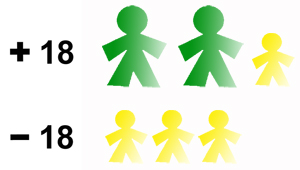
\includegraphics[scale=2]{6.jpg}
\end{figure}
\item {\bf Método poco sensible pero muy específico:} en este caso, posee poca capacidad de detectar positivos, pero alta capacidad para detectar a los negativos, es decir, no es un método muy fiable para detectar a los individuos mayores de edad, pero sí lo es para detectar a aquellos individuos que no lo son. Estos métodos tienen una elevada probabilidad de ofrecer “falsos negativos”.
\begin{figure}[h!]
\centering
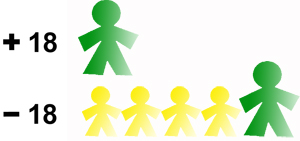
\includegraphics[scale=2]{7.jpg}
\end{figure}
\item {\bf Método poco sensible y poco específico:} posee poca capacidad para detectar tanto a los negativos como a los positivos, por lo que se trata de un método ineficaz para estimar la mayoría de edad.
\begin{figure}[h!]
\centering
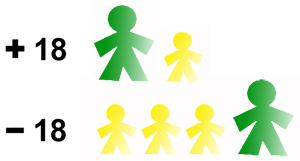
\includegraphics[scale=2]{8.jpg}
\end{figure}
\end{enumerate}
\section{Determinación de la edad en adultos}
\subsection{Sinostosis de las suturas craneales. Método de Meindi y Lovejoy.}
Las suturas craneales son las líneas articulares entre los distintos huesos que constituyen el cráneo.
\begin{figure}[h!]
\centering
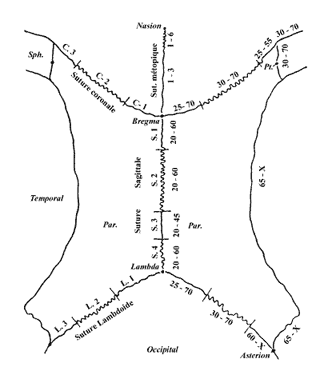
\includegraphics[scale=1]{9.png}
\caption{Edad de cierre de las suturas craneales, según el método de Vallois, modificado \cite{olivier1960pratique}.}
\end{figure}
En las primeras décadas de la vida, las suturas están rodeadas de una capa fibrosa o membrana sutural, a través de la cual se produce el crecimiento del hueso.

Cuando esta membrana queda totalmente osificada, los huesos se sueldan entre sí imposibilitando el aumento de la capacidad craneana. A pesar de que se han realizado numerosos trabajos sobre el cráneo \cite{todd1924endocranial, mckern1957skeletal, nemeskeri1960methoden},  son muchos los autores que han puesto en duda la efectividad de este método cuando se intenta establecer la edad de un individuo\cite{masset1989age}.

Aunque hay una tendencia al cierre progresivo de las suturas, es cierto que existe una gran variabilidad y se observan importantes diferencias intra e interpoblacionales. En este sentido, Genovés y Messmacher encontraron un error promedio de 11 años entre las edades estimadas y las reales de individuos mexicanos de filiación conocida \cite{genoves1959valor}.

El sistema propuesto por Meindl y Lovejoy considera la valoración conjunta del grado de sinostosis observado en dos zonas craneales. En concreto, la bóveda que incluye la zona lambdoidea media, lambda, obelion, sagital anterior, bregma, coronal media y pterion.
\newpage
Para la valoración lateral anterior hay que tener en cuenta los siguientes puntos: pterion, coronal media, esfenofrontal, y esfenotemporal inferior y superior.

En la siguiente tabla aparecen las edades medias y los rangos de edad obtenidos por medio de esta clasificación. Como los autores indican, la zona lateral anterior es más fiable que la bóveda, sobre todo para las edades avanzadas.
\begin{center}
\resizebox{13cm}{!}{
\begin{tabular}{| c | c | c | c | c | c | c |}
\hline 
\multicolumn{7}{ |c| }{{\bf Determinación de la edad mediante el cierre ectocraneal de las suturas en la parte antero-lateral}}\\
\hline 
Clasificación & N & Edad media & S.D & Desviación media & Rango interdecílico & Rango\\
\hline 0 (abierto) & 42 & & & & -43 & -50\\
\hline 1 & 18 & 32.0 & 8.3 & 6.7 & 21-42 & 19-48\\
\hline 2 & 18 & 36.2 & 6.2 & 4.8 & 29-44 & 25-49\\
\hline 3, 4, 5 & 56 & 41.1 & 10.0 & 8.3 & 28-52 & 36-68\\
\hline 6 & 17 & 43.4 & 10.7 & 8.5 & 30-54 & 23-63\\
\hline 7,  8 & 31 & 45.5 & 8.9 & 7.4 & 35-57 & 32-65\\
\hline 9, 10 & 29 & 51.9 & 12.5 & 10.2 & 39-69 & 33-76\\
\hline 11, 12, 13 & 24 & 56.2 & 8.5 &6.3 & 49-65 & 34-68\\
\hline 14 & 1 & & & & & \\
\hline 15 (cerrado) & & & & & & \\
\hline
\end{tabular}}
\end{center}

\begin{center}
\resizebox{13cm}{!}{
\begin{tabular}{| c | c | c | c | c | c | c |}
\hline 
\multicolumn{7}{ |c| }{{\bf Determinación de la edad mediante el cierre ectocraneal de las suturas de la bóveda}}\\
\hline 
Clasificación & N & Edad media & S.D & Desviación media & Rango interdecílico & Rango\\
\hline 0 (abierto) & 24 & & & & -35 & -49\\
\hline 1, 2 & 12 & 30.5 & 9.6 & 7.4 & 19-44  & 18-45\\
\hline 3, 4, 5, 6, & 30 & 34.7 & 7.8 & 6.4 & 23-45 & 22-48\\
\hline 7,  8, 9, 10 & 50 & 39.4 & 9.1 & 7.2 & 28-44 & 24-60\\
\hline 11 & 50 & 45.2 & 12.6 & 10.3 & 31-65 & 24-75\\
\hline 12, 13, 14 & 31 & 48.8 & 10.5 & 8.3 & 35-60 & 30-71\\
\hline 15 & 26 & 51.5 & 12.6 & 9.8 & 34-63 & 23-76\\
\hline 16, 17, 18  & 13 & & & & & \\
\hline 19, 20 & & & & & & \\
\hline 21 (cerrado) & & & & & & \\
\hline
\end{tabular}}
\end{center}

Recientemente, V. Galera y colaboradores compararon los métodos desarrollados por Acsádi y Nemeskéri \cite{acsadi1970history}, Baker \cite{baker1984relationship} y Meindl y Lovejoy \cite{meindl1985ectocranial}(. Para ello utilizaron 963 cráneos de la colección Terry pertenecientes a individuos blancos y negros de ambos sexos (408 blancos y 555 negros).
Para estos autores, el sistema más fiable es el de Acsadi y Nemeskeri , aunque encuentran diferencias que dependen de las distintas categorías de edad, por lo que proponen que la selección de la metodología a seguir debe estar influenciada por los indicadores postcraneales, si es que se conservan. También encuentran diferencias que dependen del sexo y el grupo racial \cite{galera1998comparison}.
\subsection{Cambios morfológicos en la sínfisis púbica. Método de Todd.}
Los cambios morfológicos que se producen en la sínfisis púbica , la región anatómica más empleada para la determinación de la edad en adultos, tienen una alta relación con las distintas etapas de la vida.

Se pueden considerar como pioneros los trabajos que Todd realizó en 1920 sobre una serie de 306 individuos masculinos. En este estudio se sistematizaron los cambios observados en la faceta articular de la sínfisis púbica y se clasificaron en las siguientes 10 fases.
\begin{itemize}
\item {\bf Fase 1 (18-19 años):} La superficie de la sínfisis es rugosa, con crestas transversales y horizontales y surcos bien marcados; no hay núcleos de osificación y los márgenes y bordes superior e inferior no están definidos.
\begin{figure}[h!]
\centering
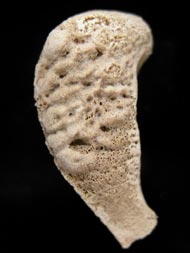
\includegraphics[scale=0.5]{f1.jpg}
\end{figure}
\item {\bf Fase 2 (20-21 años):} La superficie es todavía rugosa. Las acanaladuras horizontales comienzan a rellenarse cerca de su límite dorsal con hueso nuevo de textura fina. Pueden aparecer nódulos óseos fusionados a la parte superior y el margen dorsal comienza a delimitarse.
\begin{figure}[h!]
\centering
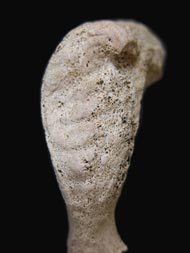
\includegraphics[scale=0.5]{f2.jpg}
\end{figure}
\item {\bf Fase 3 (22-24 años):} La superficie de la sínfisis muestra una progresiva obliteración del sistema de crestas y surcos. Comienza la formación de una plataforma dorsal; puede haber nódulos óseos. Definición del margen dorsal que aparece ligeramente elevado ya que el bisel ventral es más pronunciado. Los extremos no están delimitados.
\newpage
\begin{figure}[h!]
\centering
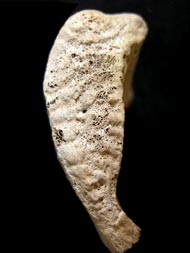
\includegraphics[scale=0.5]{f3.jpg}
\end{figure}
\item {\bf Fase 4 (25-26 años):} Gran incremento del área biselada ventral y una correspondiente disminución del sistema de crestas y surcos. Completa definición del margen dorsal a través de la formación de la plataforma dorsal. Se inicia la delimitación del extremo inferior.
\begin{figure}[h!]
\centering
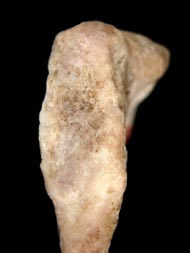
\includegraphics[scale=0.5]{f4.jpg}
\end{figure}
\item {\bf Fase 5 (27-30 años):} Hay pocos cambios en la superficie de la sínfisis y en la plataforma dorsal. Los márgenes están claramente definidos y ligeramente labiados. La extremidad inferior está mejor definida y la superior está en formación, con o sin la presencia de un nódulo óseo.
\begin{figure}[h!]
\centering
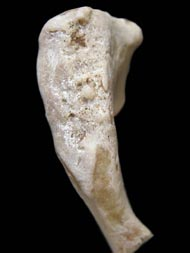
\includegraphics[scale=0.5]{f5.jpg}
\end{figure}
\item {\bf Fase 6 (30-35 años):} Incremento de la definición de los extremos. Desarrollo casi completo de la rampa ventral ventral. La retención de alguna textura granular en la superficie de la sínfisis indica que la actividad no ha cesado todavía. Las características del aspecto ventral, en la zona adyacente al reborde comienzan a transformarse en una cara compacta. El reborde puede estar ya algo indefinido. No hay levantamiento del margen ventral y no aumenta el del margen dorsal.
\begin{figure}[h!]
\centering
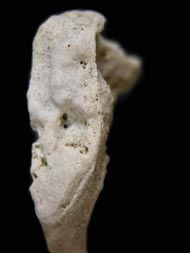
\includegraphics[scale=0.5]{f6.jpg}
\end{figure}
\item {\bf Fase 7 (35-39 años):} Hay cambios en el aspecto de la superficie y zona ventral, que pasa desde granular a granulado fino o hueso denso. Los cambios son ligeros en la superficie de la sínfisis y marcados en la zona ventral por la disminución de su actividad. No hay formación de bordes en la sínfisis. No hay osificación de tendones ni inserciones ligamentosas. Hay cambios en el aspecto de la superficie y zona ventral, que pasa desde granular a granulado fino o hueso denso. Los cambios son ligeros en la superficie de la sínfisis y marcados en la zona ventral por la disminución de su actividad. No hay formación de bordes en la sínfisis. No hay osificación de tendones ni inserciones ligamentosas.
\begin{figure}[h!]
\centering
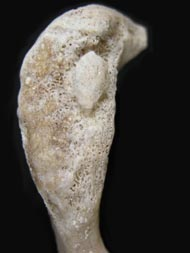
\includegraphics[scale=0.5]{f7.jpg}
\end{figure}
\item {\bf Fase 8 (40-45 años):} La superficie de la sínfisis y el aspecto ventral está generalmente suavizado e inactivo. El anillo oval está completo. No hay un levantamiento marcado de los márgenes ventral ni dorsal. Extremos claramente definidos y no hay acanaladuras en la sínfisis. Desarrollo de la osificación de inserciones tendinosas y ligamentosas especialmente del 'ligamentum sacrotuberale' y el 'musculus gracilis'.
\begin{figure}[h!]
\centering
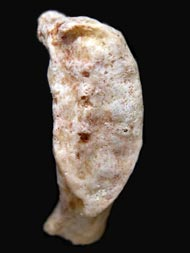
\includegraphics[scale=0.5]{f8.jpg}
\end{figure}
\item {\bf Fase 9 (45-49 años):} La faceta muestra un borde más o menos marcado. El margen dorsal está labiado uniformemente y el ventral de manera irregular.
\begin{figure}[h!]
\centering
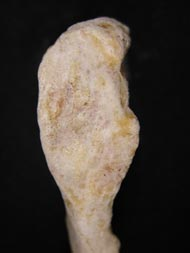
\includegraphics[scale=0.5]{f9.jpg}
\end{figure}
\item {\bf Fase 10 (más de 50 años):} Rarefacción de la superficie y osificación irregular. Incremento de la desfiguración conforme aumenta la edad.
\begin{figure}[h!]
\centering
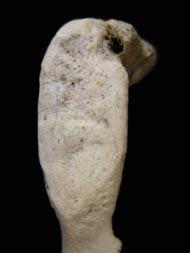
\includegraphics[scale=0.5]{f10.jpg}
\end{figure}
\end{itemize}
Trabajos posteriores demostraron que esta clasificación de Todd no era del todo exacta si se aplicaba a individuos femeninos, ya que en estos casos se le asignaban a los sujetos edades superiores a las que realmente tenían.

Como afirmó Stewart, existen claras diferencias sexuales, ya que los cambios en la morfología de la sínfisis púbica se producen a un ritmo más acelerado en las mujeres que en los hombres. Por otra parte, también se observaron deficiencias al determinar la edad de individuos entre los 20 y 40 años \cite{hanihara1978estimation, suchey1979problems}
\subsection{Estimación de la edad dental}
En 1992, Lamendin et al. desarrollaron una técnica para la estimación de la edad en individuos adultos utilizando dientes monoradiculares (incisivos, caninos y premolares) extraídos de su alveolo. La técnica se basa en la medición de dos factores relacionados con la edad: (i) la regresión gingival o periodontosis, y (ii) la trasparencia radicular.

La periodontosis es debida a la degeneración de los tejidos blandos del diente, progresando desde la línea amelocementaria hasta el ápice dental. Por otro lado, la transparencia radicular se debe al depósito de cristales de hidroxiapatita de calcio en el interior de los túbulos dentinarios, cambiando así el índice refractario de la dentina radicular.
Se miden las siguientes distancias en la superficie vestibular del diente:
\begin{itemize}
\item Altura de la raíz (AR): distancia directa desde el ápice hasta la unión amelocementaria.
\item Altura de la periodontosis (AP): distancia directa entre la unión amelocementaria y el nivel de la colocación del periodonto.
\item Altura de la transparencia de la raíz (ATR): distancia directa desde el ápice de la raíz hasta el punto de división entre la parte traslúcida y no traslúcida. Esta característica se observa con la ayuda de un negatoscopio.
\end{itemize}
Con estas mediciones se calculan los siguientes parámetros:
\begin{center}
$P=\frac{AP}{AR}\times 100$
$T=\frac{ATR}{AR}\times 100$
\end{center}
que son los utilizados para la estimación de la edad mediante el uso de la siguiente fórmula de regresión:
\begin{center}
$Edad=(0,18\times P)+(0,42\times T)+25,53$
\end{center}
Prince y Ubelaker en 2002 mejoraron la metodología propuesta originalmente por Lamendin et al., desarrollando fórmulas de regresión diferenciadas por sexos y grupo ancestral. Las ecuaciones para población desarrolladas para población caucasoide son las siguientes:
\begin{center}
Mujeres: $Edad=(1,10\times AR)+(0,31\times P)+(0,39\times T)+11,82$\\
Varones: $Edad=(0,15\times AR)+(0,29\times P)+(0,39\times T)+23,17$
\end{center}
Las fórmulas propuestas por Prince y Ubelaker tienen un margen de error promedio de 8,2 años, alcanzándose una mayor precisión entre individuos de entre 30–69 años. Por debajo de los 30 años se produce una sobreestimación de la edad, mientras que por encima de los 69 años se produce una infraestimación.
\newpage
\bibliography{Biblio}
\end{document}